\chapter{Introduction}

\subsubsection{Motivation}
 
Radial image reconstruction is widely used today in computational imaging, such as in Computerized Tomography (CT) scans, which are essential for diagnosing diseases or injuries. The use of such CT scans has increased drastically, making this a domain worthy of exploring optimization techniques.

The mathematics community continues to engage with these problems, exploring the Fourier transform and the Radon transform, the latter of which we also use in this thesis.

Moreover, artists must intuitively find an arrangement of the string that can recreate a given image. This process can be very tedious and time-consuming, which is why we will tackle the problem of finding a mathematical method for computing string art, thus automating the process.

\subsubsection{Personal Contribution}

In the course of this thesis we read existing literature on string art \cite{towards-computational-stringart} and \cite{computational-stringart} as well as computational optimization techniques \cite{convex-optimization}. In addition, we implemented several optimization algorithms and adapted the well known Radon transform specifically for the string art context. We designed and executed experiments to evaluate the performance of these methods and the visual quality of the results, analyzing each algorithm's strengths and limitations. Additionally, we implemented a Python package containing all the methods and experiments, ensuring the reproducibility of the results through clear documentation and organized code.

\subsubsection{Structure}

We will begin by establishing a foundation of mathematical formulas and concepts in the \textit{Preliminary} section, which will serve as the basis for the methods presented later. Next, we will explore all of the optimization algorithms implemented in the \textit{Methodology} chapter. Finally, we will conclude with a summary and a discussion of potential directions for future work.

\subsubsection{Digital Interpretation of String Art}

String art is a technique for creating a visual effect by manipulating thread to reproduce an image. We will procedurally compute string art configurations from a given image, modeling this real world problem using mathematical constraints.

The objective is to replicate this effect digitally, given an input image. It is important to note that there are a multiple of methods to achieve this objective, and we will examine the more intricate details of each approach.

The definition of string art we addressed earlier will not be fully applicable when recreating the image digitally, meaning some of the original constraints will be relaxed in order to explore the possibilities and limitations of this domain. This is because our objective is to visually replicate the effect produced by the traditional method, without being limited by physical constraints, such as the use of a continuous thread.

\begin{figure}[!htb]
    \centering
    \begin{minipage}{0.48\linewidth}
        \centering
        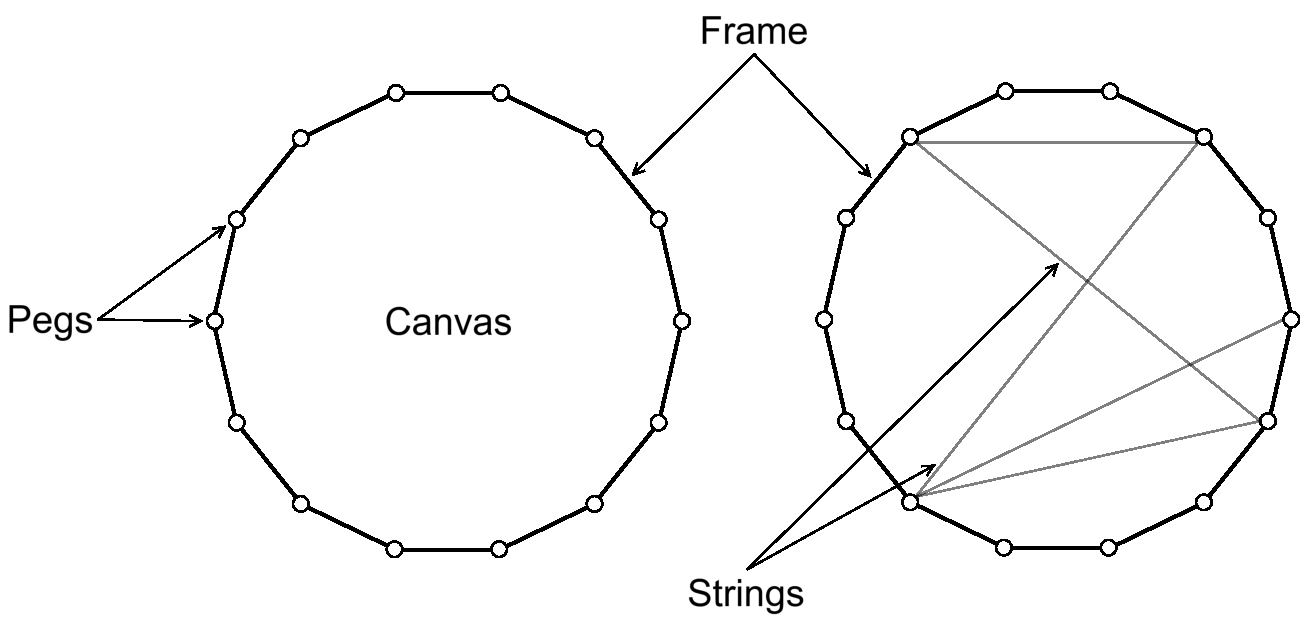
\includegraphics[width=\linewidth]{images/stringart_components.pdf}
        \caption{Image to illustrate the main components involved in creating string art patterns.}
        \label{fig:stringart_components}
    \end{minipage}
    \hfill
    \begin{minipage}{0.48\linewidth}
        \centering
        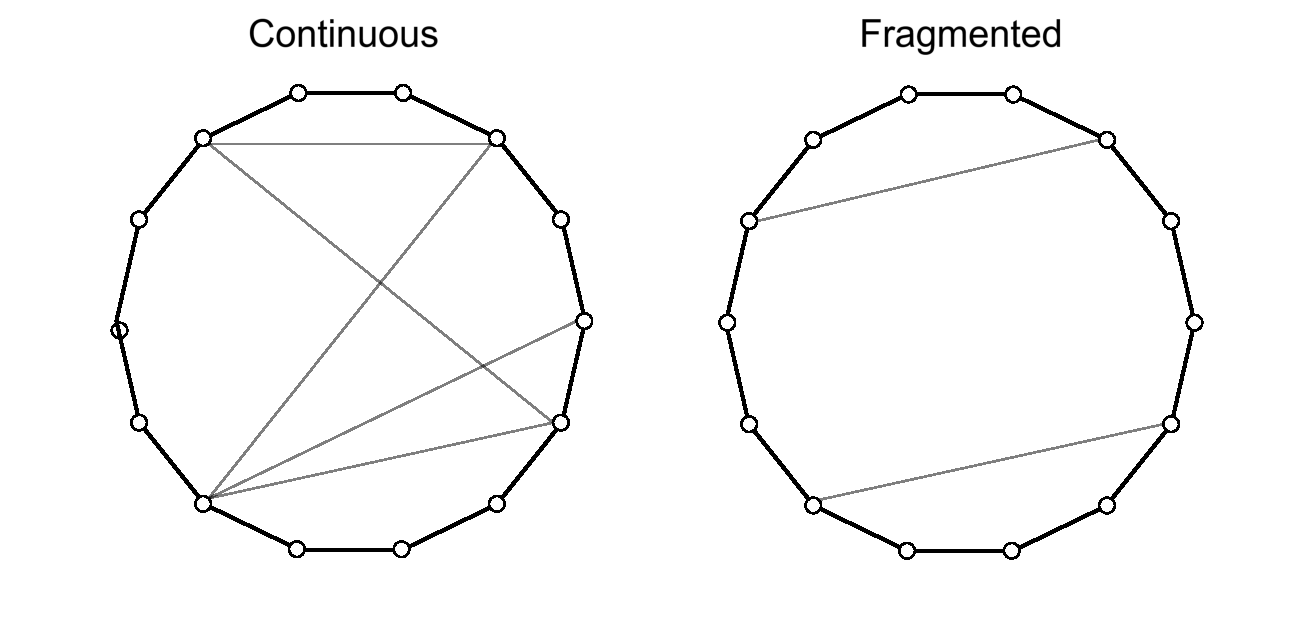
\includegraphics[width=\linewidth]{images/continuous_vs_fragmented.pdf}
        \caption{Image to illustrate the different types of arrangements: continuous versus fragmented.}
        \label{fig:continuous_vs_fragmented_strings}
    \end{minipage}
\end{figure}

Even though we are limited to drawing only straight lines, we can create the effect of a curve by drawing multiple lines that follow the trajectory of a quadratic Bézier curve. The image below illustrates this behavior.

\begin{figure}[H]
    \centering
    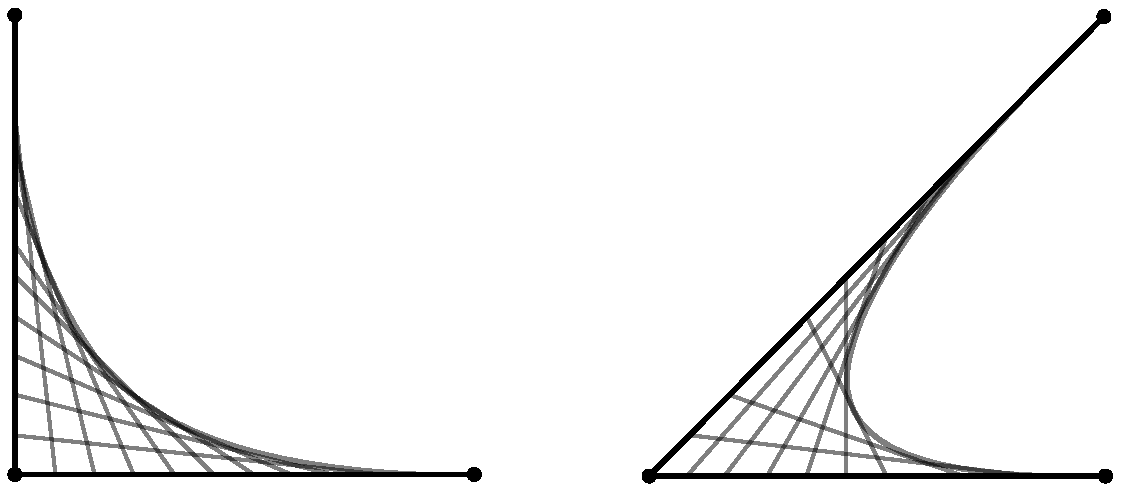
\includegraphics[width=0.5\linewidth]{images/quadratic_bezier_curves.pdf}
    \caption{Illustration of quadratic Bézier curves approximated by straight lines.}
    \label{fig:bezier_cureves}
\end{figure}